% -*- coding: latin-1; -*-
\documentclass{book}

\usepackage[T1]{fontenc}
\usepackage[latin1]{inputenc}
\usepackage{color}
\usepackage{epsfig}
\usepackage{alltt}
\usepackage{moreverb}

\ifx\pdfoutput\undefined \csname newcount\endcsname\pdfoutput \fi 
\ifcase\pdfoutput  \else 
\usepackage[pdftex]{hyperref}
\fi

\setlength{\parskip}{0.3cm}
\setlength{\parindent}{0cm}

\def\inputfig#1{\input #1}

\newenvironment{itemize0}{
\begin{itemize}
\setlength{\parskip}{0cm}%
}
{\end{itemize}}

\newenvironment{enumerate0}{
\begin{enumerate}
\setlength{\parskip}{0cm}%
}
{\end{enumerate}}

\input spec-macros

\newcommand{\gloss}[1]{\textsl{\textcolor{red}{#1}}}
\newcommand{\glossentry}[1]{\paragraph{#1}}
\newcommand{\class}[1]{\texttt{#1}}
\newcommand{\genfun}[1]{\texttt{#1}}
\newcommand{\macro}[1]{\texttt{#1}}
\newcommand{\gadget}[1]{\texttt{#1}}
\newcommand{\pane}[1]{\texttt{#1}}
\newcommand{\initarg}[1]{\texttt{#1}}
\newcommand{\methcomp}[1]{\texttt{#1}}
\newcommand{\slot}[1]{\texttt{#1}}
\newcommand{\code}[1]{\texttt{#1}}

\newcommand{\longref}[1]{(See \ref{#1})}
\newcommand{\var}[1]{\textit{#1}}

\newcommand{\nil}[0]{\cl{nil}}
\title{McCLIM 0.01 user's manual}
\author{Robert Strandh \\ strandh@labri.fr}

\begin{document}
\maketitle

{\setlength{\parskip}{0cm}
\tableofcontents}

\chapter{Introduction}

CLIM is a large layered software system that allows the user to
customize it at each level.  The most simple ways of using CLIM is to
directly use its top layer, which contains application frames, panes,
and gadgets, very similar to those of traditional windowing system
toolkits such as GTK, Tk, and Motif.

But there is much more to using CLIM.  In CLIM, the upper layer with
panes and gadgets is written on top of a basic layer containing more
basic functionality in the form of sheets.  Objects in the upper layer
are typically instances of classes derived from those of the lower
layer.  Thus, nothing prevents a user from adding new gadgets and
panes by writing code that uses the sheet layer.

Finally, since CLIM is written in Common Lisp, essentially all parts
of it can be modified, replaced, or extended.

For that reason, a user's manual for CLIM must contain not only a
description of the protocols of the upper layer, but also of all
protocols, classes, functions, macros, etc. that are part of the
specification.

\section{Standards}
This manual documents McCLIM 0.01 which is a mostly complete implementation of
the CLIM~2.0 specification and its revision~2.2. To our knowledge
version~2.2 of the CLIM specification is only documented in the ``CLIM~2
User's Guide'' by Franz. While that document is not a formal
specification, it does contain many cleanups and is often clearer than
the official specification; on the other hand, the original
specification is a useful reference. This manual will note where
McCLIM has followed the 2.2 API.

Also, some protocols mentioned in the 2.0 specification, such as parts
of the incremental redisplay protocol, are clearly internal to CLIM
and not well described.  It will be noted here when they are partially
implemented in McCLIM or not implemented at all.

\part{Getting Started}

\chapter{CLIM Demos and Applications}

\section{Running the Demos}

The McCLIM source distribution comes with a number of demos and
applications.  They are intended to showcase specific CLIM features,
demonstrate programming techniques or provide useful tools.

These demos and applications are available in the \texttt{Examples}
and \texttt{Apps} subdirectories of the source tree's root directory.
Instructions for compiling, loading and running some of the demos are
included in the files with the McCLIM installation instructions for
your Common Lisp implementation. See for example the file
\texttt{INSTALL} if you use Allegro CL, \texttt{INSTALL.CMU} for
CMUCL, \texttt{INSTALL.OPENMCL} for OpenMCL, and so on.

Below is a complete list of the McCLIM demos and applications, sorted
in alphabetical order.  Each entry provides a short description of
what the program does, with instructions for compiling and running it
if not mentioned in the general installation instructions.

\begin{description}
\item[\texttt{Apps/Listener}] CLIM-enabled Lisp listener.  See the
compilation and execution instructions in
\texttt{Apps/Listener/README}.
\item[\texttt{Examples/address-book.lisp}] Simple address book.  See
McCLIM's installation instructions.
\item[\texttt{Examples/calculator.lisp}] Simple desk calculator.  See
McCLIM's installation instructions.
\item[\texttt{Examples/clim-fig.lisp}] Simple paint program.  You can
run it by evaluating this form at the Lisp prompt:
\begin{verbatim}
(clim-demo::clim-fig)
\end{verbatim}
\item[\texttt{Examples/colorslider.lisp}] Interactive color editor.
See McCLIM's installation instructions.
\item[\texttt{Examples/demodemo.lisp}] Demonstrates different pane
types.  You can compile it by evaluating:
\begin{verbatim}
(compile-file "Examples/demodemo.lisp")
\end{verbatim}
Then load it with:
\begin{verbatim}
(load "Examples/demodemo")
\end{verbatim}
Finally, run it with:
\begin{verbatim}
(clim-demo::demodemo)
\end{verbatim}
\item[\texttt{Examples/goatee-test.lisp}] Text editor with Emacs-like
key bindings.  See McCLIM's installation instructions.
\item[\texttt{Examples/menutest.lisp}] Displays a window with a simple
menu bar.  See McCLIM's installation instructions.
\item[\texttt{Examples/postscript-test.lisp}] Displays text and
graphics to a PostScript file.  Run it with:
\begin{verbatim}
(clim-demo::postscript-test)
\end{verbatim}
The resulting file \texttt{ps-test.ps} is generated in the current
directory and can be displayed by a PostScript viewer such as
\texttt{gv} on Unix-like systems.
\item[\texttt{Examples/presentation-test.lisp}] Displays an
interactive window in which you type numbers that are successively
added.  When a number is expected as input, you can either type it at
the keyboard, or click on a previously entered number. Run it with:
\begin{verbatim}
(clim:run-frame-top-level (clim:make-application-frame
                           'clim-demo::summation))
\end{verbatim}
\item[\texttt{Examples/sliderdemo.lisp}] Apparently a calculator demo
(see above).  Compile with:
\begin{verbatim}
(compile-file "Examples/sliderdemo.lisp")
\end{verbatim}
Load with:
\begin{verbatim}
(load "Examples/sliderdemo")
\end{verbatim}
Run with:
\begin{verbatim}
(clim-demo::slidertest)
\end{verbatim}
\item[\texttt{Examples/stream-test.lisp}] Interactive command
processor that echoes its input.  Run with:
\begin{verbatim}
(clim-demo::run-test)
\end{verbatim}
\end{description}

The following programs are currently \textbf{known not to work}:
\begin{itemize}
\item \texttt{Examples/fire.lisp}
\item \texttt{Examples/gadget-test-kr.lisp}
\item \texttt{Examples/gadget-test.lisp}
\item \texttt{Examples/puzzle.lisp}
\item \texttt{Examples/traffic-lights.lisp}
\item \texttt{Examples/transformations-test.lisp}
\end{itemize}

\section{McCLIM Installation and Usage Tips}

This section collects useful installation and usage tips.  They refer
to specific Common Lisp implementations or McCLIM features.

\subsection{Multiprocessing with CMUCL}

Before beginning a McCLIM session with CMUCL, \textbf{you are strongly
advised} to initialize multiprocessing by evaluating the form:
\begin{verbatim}
(mp::startup-idle-and-top-level-loops)
\end{verbatim}
If you use the SLIME development environment under Emacs, evaluate the
above form from the \texttt{*inferior-lisp*} buffer, not from
\texttt{*slime-repl[n]*}.  Initializing multiprocessing can make a
difference between an application that starts instantaneously on, say,
a Pentium IV class PC, and one that may take \emph{minutes} on the
same machine.

\subsection{Pointer Documentation: Adding Mouse Button Icons}

McCLIM comes with experimental code for adding graphical mouse button
icons to pointer documentation panes.  To use this feature, you have
to first compile the file \texttt{Experimental/pointer-doc-hack.lisp}
in the source tree.  Assuming you have built McCLIM from source as
explained in the installation instructions, evaluate this form to
compile the file:
\begin{verbatim}
(compile-file "Experimental/pointer-doc-hack.lisp")
\end{verbatim}
Then, to activate the feature, load the compiled file before starting
a McCLIM session or application:
\begin{verbatim}
(load "Experimental/pointer-doc-hack")
\end{verbatim}
Alternatively, you may dump a Lisp image containing McCLIM and the
graphical pointer documentation code.  See the documentation of your
Common Lisp system for more information.

\chapter{The First Application}

\section{Panes and Gadgets}

A CLIM application is made up of a hierarchy of \gloss{panes} and
\gloss{gadgets} (gadgets are special kinds of panes).  These elements
correspond to what other toolkits call \emph{widgets}.
Frequently used CLIM gadgets are \gadget{button}s, \gadget{slider}s,
etc, and typical panes are the layout panes such as \pane{hbox},
\pane{vbox}, \pane{hrack}, etc.

\section{Defining Application Frames}

Each CLIM application is defined by an \gloss{application frame}.  An
application frame is an instance of the class
\class{application-frame}.  As a CLIM user, you typically define a
class that inherits from the class \class{application-frame}, and
that contains additional slots needed by your application.  It is
considered good style to keep all your application-specific data in
slots in the application frame (rather than, say, in global
variables), and to define your application-specific application frame
in its own package.  

The usual way to define an application frame is to use the macro
\macro{define-application-frame}.  This macro works much like
\macro{defclass}, but also allows you to specify the hierarchy of
\gloss{panes} and \gloss{gadgets} to use. 

\section{A First Attempt}

Let us define a very primitive CLIM application.  For that, let us put
the following code in a file:

\verbatimtabinput{ex1.lisp}

As we can see in this example, we have put our application in a
separate package, here a package named \texttt{APP}.  While not
required, putting the application in its own package is good practice.  

The package for the application uses two packages: \texttt{CLIM} and
\texttt{CLIM-LISP}.  The \texttt{CLIM} package is the one that
contains all the symbols needed for using CLIM.  The
\texttt{CLIM-LISP} package replaces the \texttt{COMMON-LISP} package
for CLIM applications.  It is essentially the same as the
\texttt{COMMON-LISP} package as far as the user is concerned.

In our example, we export the symbol that corresponds to the main
function to start our application, here called \texttt{APP-MAIN}. 

The most important part of the code in our example is the definition
of the application-frame.  In our example, we have defined an
application frame called \texttt{superapp}, which becomes a CLOS class
that automatically inherits from some standard CLIM application frame
class.

The second argument to \texttt{define-application-frame} is a
list of additional superclasses from which you want your application
frame to inherit.  In our example, this list is empty, which means
that our application frame only inherits from the standard CLIM
application frame.  

The third argument to \texttt{define-application-frame} is a list of
CLOS slots to be added to any instance of this kind of application
frame.  These slots are typically used for holding all
application-specific data.  The current instance if the application
frame type will always be the value of the special variable
\texttt{*application-frame*}, so that the values of these slots can be
accessed.  In our example, we do not initially have any further
slots. 

The rest of the definition of an application frame contains additional
elements that CLIM will allow the user to define.  In our example, we
have two additional (mandatory) elements: \texttt{:panes} and
\texttt{:layouts}.  

The \texttt{:panes} element defines a collection of CLIM panes that
each instance of your application may have.  Each pane has a name, a
type, and perhaps some options that are used to instantiate that
particular type of pane.  Here, we have a pane called \texttt{int} of
type \texttt{:interactor} with a height of 400 units and a width of
600 units.  In McCLIM, the units are initially physical units (number
of pixels) of the native windowing system.

The \texttt{:layouts} element defines one or more ways of organizing
the panes in a hierarchy.  Each layout has a name and a description of
a hierarchy.  In our example, only one layout, named \texttt{default},
is defined.  The layout called \texttt{default} is the one that is
used by CLIM at startup.  In our example, the corresponding hierarchy
is trivial, since it contains only the one element \texttt{int}, which
is the name of our only pane. 

\section{Executing the Application}

In order to run a CLIM application, you must have a Lisp system that
contains McCLIM.  If you use CMUCL or SBCL, you either need a
\texttt{core} file that already has McCLIM in it, or else, you have to
load the McCLIM compiled files that make up the McCLIM distribution.
The fist solution is recommended so as to avoid having to load the
McCLIM files each time you start your CLIM application. 

To execute the application, load the file containing your code
(possibly after compiling it) into your running Lisp system.  Then
start the application.  Our example can be started by typing
\texttt{(app:app-main)}. 

\section{Adding Functionality}

In a serious application, you would probably want some area where your
application objects are to be displayed.  In CLIM, such an area is
called an \emph{application pane}, and would be an instance (direct
or indirect) of the CLIM class \texttt{application-pane}.
In fact, instances of this class are in reality also \emph{streams}
which can be used in calls both to ordinary input and output functions
such as \texttt{format} and \texttt{read} and to CLIM-specific
functions such as \texttt{draw-line}.

In this example we have such an application pane, the name of which is
\texttt{app}.  As you can see, we have defined it with an option
\texttt{:display-time nil}.  The default value for this option for an
application pane is \texttt{:command-loop}, which means that the pane
is cleared after each iteration in the command loop, and then
redisplayed using a client-supplied \emph{display function}.  The
default display function does nothing, and we have not supplied any,
so if we had omitted the \texttt{:display-time nil} option, the
\texttt{parity} command would have written to the pane.  Then, at the
end of the command loop, the pane would have been cleared, and nothing
else would have been displayed.  The net result is that we would have
seen no visible output.  With the option \texttt{:display-time nil},
the pane is never cleared, and output is accumulated every time we
execute the \texttt{parity} command.


For this example, let us also add a few \emph{commands}.  Such
commands are defined by the use of a macro called
\texttt{define-}\textit{name}\texttt{-command}, where \textit{name} is
the name of the application, in our case \texttt{superapp}. This macro
is automatically defined by \texttt{define-application-frame}.  

Let us also add a pane that automatically provides documentation for
different actions on the pointer device. 

Here is our improved example:

\verbatimtabinput{ex2.lisp}

If you execute this example, you will find that you now have three
different panes, the application pane, the interactor pane and the
pointer documentation pane.  In the pointer documentation pane, you
will see the text \texttt{R possibilities} which indicates that if you
click the right mouse button, you will automatically see a popup menu
that lets you choose a command.  In our case, you will have the
default commands that are automatically proposed by McCLIM plus the
commands that you defined yourself, in this case \texttt{quit} and
\texttt{parity}. 

Figure \ref{figex2} shows what ought to be visible on the screen. 

\begin{figure}
\begin{center}
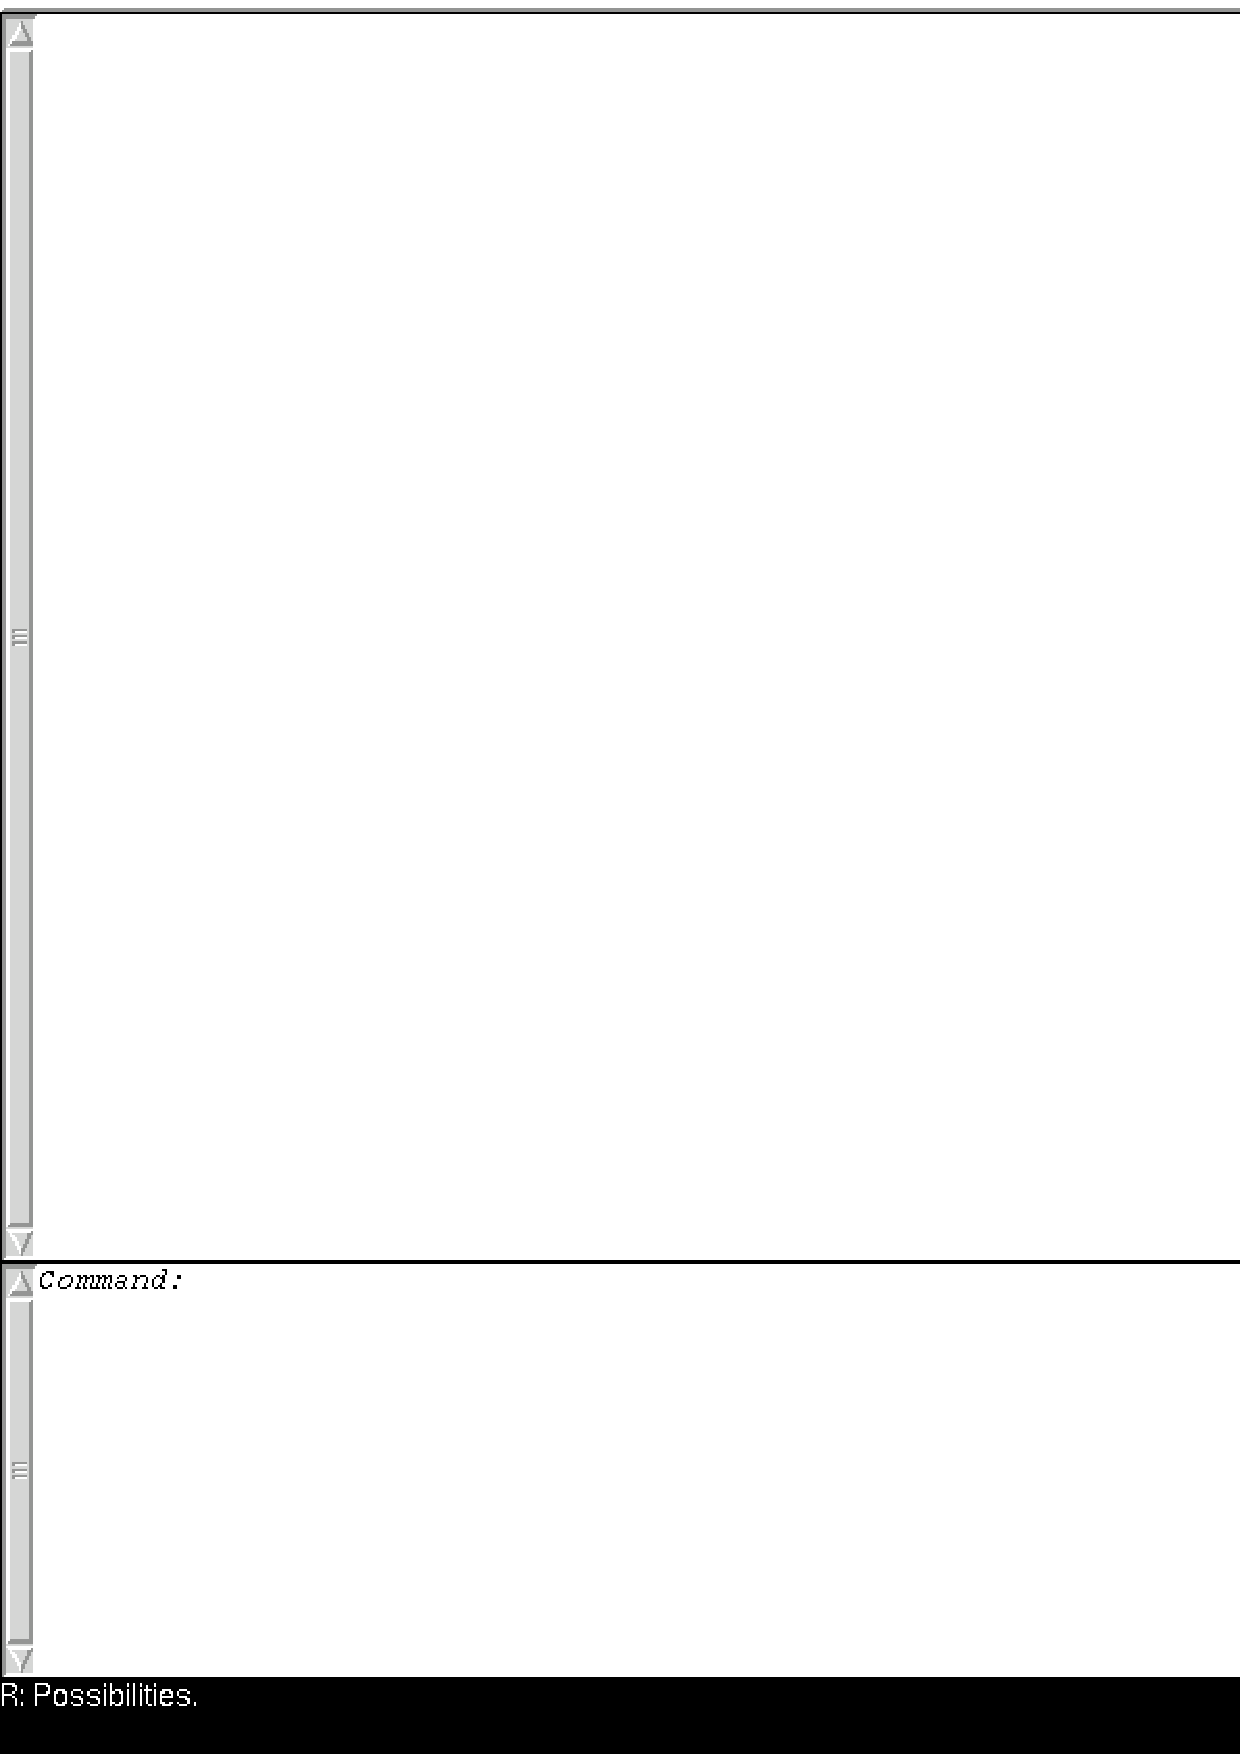
\includegraphics{ex2}
\end{center}
\caption{\label{figex2} View of the improved example}
\end{figure}

Notice that commands, in order to be available from the command line,
must have an option of \texttt{:name t}.  The reason is that some
commands will be available only from menus or by some other mechanism. 

\chapter{Using presentation types}

\section{What is a presentation type}

The concept of \emph{presentation types} is central to CLIM.  Client
code can choose to output graphical or textual representations of
application objects either as just graphics or text, or to associate
such output with an arbitrary Common Lisp object and a presentation
type.  The presentation type is not necessarily related to the idea
Common Lisp might have of the underlying object.

When a CLIM command or some other client code requests an object (say
as an argument) of a certain presentation type, the user of the
application can satisfy the request by clicking on any visible output
labeled with a compatible presentation type.  The command then
receives the underlying Common Lisp object as a response to the
request. 

CLIM presentation types are usually distinct from Common Lisp types.
The reason is that the Common Lisp type system, although very
powerful, is not quite powerful enough to represent the kind of
relationships between types that are required by CLIM.  However, every
Common Lisp class (except the built-in classes) is automatically a
presentation type.

A presentation type has a name, but can also have one or more
\emph{parameters}.  Parameters of presentation types are typically used
to restrict the type.  For instance, the presentation type
\texttt{integer} takes as parameters the low and the high values of an
interval.  Such parameters allow the application to restrict objects
that become clickable in certain contexts, for instance if a date in
the month of March is requested, only integers between 1 and 31 should
be clickable. 

\section{A simple example}

Consider the following example:

\verbatimtabinput{ex3.lisp}

In this application, we have two main panes, an application pane and
an interactor pane.  The application pane is given the option
\texttt{:display-time t} which means that it will not be erased before
every iteration of the command loop.  

We have also defined two presentation types: \texttt{name-of-month}
and \texttt{day-of-month}.  The \texttt{out} command uses
\texttt{with-output-as-presentation} in order to associate some
output, a presentation type, and an underlying object.  In this case,
it will show the string ``March'' which is considered to be of
presentation type \texttt{name-of-month} with the underlying object
being the character string \texttt{"The third month"}.  It will also
show the string ``fifteen'' which is considered to be of presentation
type \texttt{day-of-month} with the underlying object being the number
15.  The argument \texttt{t} to \texttt{with-output-as-presentation}
indicates that the stream to present on is
\texttt{*standard-output*}. 

Thus, if the \texttt{out} command has been executed, and then the user
types ``Get Date'' in the interactor pane, the \texttt{get-date}
command will try to acquire its arguments, the first of presentation
type \texttt{name-of-month} and the second of type
\texttt{day-of-month}.  At the first prompt, the user can click on the
string ``March'' but not on the string ``fifteen'' in the application
pane.  At the second prompt it is the string ``fifteen'' that is
clickable, whereas ``March'' is not.  

The \texttt{get-date} command will acquire the underlying objects.
What is finally displayed (in the interactor pane, which is the
standard input of the frame), is ``the 15 of The third month''.

\part{Reference Manual}

\chapter{Concepts}

\section{Coordinate systems}

CLIM uses a number of different coordinate systems and transformations
to transform coordinates between them.

The coordinate system used for the arguments of drawing functions is
called the \gloss{user coordinate system}, and coordinate values
expressed in the user coordinate system are known as \gloss{user
coordinates}.

Each sheet has its own coordinate system called the \gloss{sheet
coordinate system}, and positions expressed in this coordinate system
are said to be expressed in \gloss{sheet coordinates}.  User
coordinates are translated to \gloss{sheet coordinates} by means of
the \gloss{user transformation} also called the \gloss{medium
transformation}.  This transformation is stored in the \gloss{medium}
used for drawing.  The medium transformation can be composed
temporarily with a transformation given as an explicit argument to a
drawing function.  In that case, the user transformation is
temporarily modified for the duration of the drawing.

Before drawing can occur, coordinates in the sheet coordinate system
must be transformed to \gloss{native coordinates}, which are
coordinates of the coordinate system of the native windowing system.
The transformation responsible for computing native coordinates from
sheet coordinates is called the \gloss{native transformation}.  Notice
that each sheet potentially has its own native coordinate system, so
that the native transformation is specific for each sheet.  Another
way of putting it is that each sheet has a mirror, which is a window
in the underlying windowing system.  If the sheet has its own mirror,
it is the \emph{direct mirror} of the sheet.  Otherwise its mirror is
the direct mirror of one of its ancestors.  In any case, the native
transformation of the sheet determines how sheet coordinates are to be
translated to the coordinates of that mirror, and the native
coordinate system of the sheet is that of its mirror. 

The composition of the user transformation and the native
transformation is called the \gloss{device transformation}.  It allows
drawing functions to transform coordinates only once before obtaining
native coordinates. 

Sometimes, it is useful to express coordinates of a sheet in the
coordinate of its parent.  The transformation responsible for that is
called the \gloss{sheet transformation}.  

\section{Arguments to drawing functions}

Drawing functions are typically called with a sheet as an argument.

A sheet often, but not always, corresponds to a window in the
underlying windowing system.  

\chapter{Windowing system drawing functions}

A typical windowing system provides a hierarchy of rectangular areas
called windows.  When a drawing functions is called to draw an object
(such as a line or a circle) in a window of such a hierarchy, the
arguments to the drawing function will include at least the window and
a number of coordinates relative to (usually) the upper left corner of
the window.

To translate such a request to the actual altering of pixel values in
the video memory, the windowing system must translate the coordinates
given as argument to the drawing functions into coordinates relative
to the upper left corner of the entire screen.  This is done by a
composition of translation transformations applied to the initial
coordinates.  These transformations correspond to the position of each
window in the coordinate system of its parent. 

Thus a window in such a system is really just some values indicating
its height, its width, and its position in the coordinate system of
its parent, and of course information about background and foreground
colors and such.

\chapter{CLIM drawing functions}

CLIM generalizes the concept of a hierarchy of window in a windowing
system in several different ways.  A window in a windowing system
generalizes to a \gloss{sheet} in CLIM.  More precisely, a window in a
windowing system generalizes to the \gloss{sheet region} of a sheet.
A CLIM sheet is an abstract concept with an infinite \gloss{drawing
plane} and the \gloss{region} of the sheet is the potentially visible
part of that drawing plane. 

CLIM \gloss{sheet region}s don't have to be rectangular the way
windows in most windowing systems have to be.  Thus, the width and the
height of a window in a windowing system generalizes to an arbitrary
\gloss{region} in CLIM.  A CLIM region is simply a set of mathematical
points in a plane.  CLIM allows this set to be described as a
combination (union, intersection, difference) of elementary regions
made up of rectangles, polygons and ellipses. 

Even rectangular regions in CLIM are generalizations of the
width+height concept of windows in most windowing systems.  While the
upper left corner of a window in a typical windowing system has
coordinates (0,0), that is not necessarily the case of a CLIM region.
CLIM uses that generalization to implement various ways of scrolling
the contents of a sheet.  To see that, imagine just a slight
generalization of the width+height concept of a windowing system into
a rectangular region with x+y+width+height.  Don't confuse the x and y
here with the position of a window within its parent, they are
different.  Instead, imagine that the rectangular region is a hole
into the (infinite) drawing plane defined by all possible coordinates
that can be given to drawing functions.  If graphical objects appear
in the window with respect to the origin of some coordinate system,
and the upper-left corner of the window has coordinates (x,y) in that
coordinate system, then changing x and y will have the effect of
scrolling. 

CLIM sheets also generalize windows in that a window typically has
pixels with integer-value coordinates.  CLIM sheets, on the other
hand, have infinte resolution.  Drawing functions accept non-integer
coordinate values which are only translated into integers just before
the physical rendering on the screen.

The x and y positions of a window in the coordinate system of its
parent window in a typical windowing system is a translation
transformation that takes coordinates in a window and transform them
into coordinates in the parent window.  CLIM generalizes this concepts
to arbitrary affine transformations (combinations of translations,
rotations, and scalings).  This generalization makes it possible for
points in a sheet to be not only translated compared to the parent
sheet, but also rotated and scaled (including negative scaling, giving
mirror images).  A typical use for scaling would be for a sheet to be
a zoomed version of its parent, or for a sheet to have its
y-coordinate go the opposite direction from that of its parent. 

When the shapes of, and relationship between sheets are as simple as
those of a typical windowing system, each sheet typically has an
associated window in the underlying windowing system.  In that case,
drawing on a sheet translates in a relativly straightforward way into
drawing on the corresponding window.  CLIM sheets that have associated
windows in the underlying windowing system are called \gloss{mirrored
sheets} and the system-dependent window object is called the
\gloss{mirror}.  When shapes and relationships are more complicated,
CLIM uses its own transformations to transform coordinates from a
sheet to its parent and to its grandparent, etc., until a
\gloss{mirrored sheet} is found.  To the user of CLIM, the net effect
is to have a windowing system with more general shapes of, and
relationships between windows.


\chapter{Sheet hierarchy}

CLIM sheets are organized into a hierarchy.  Each sheet has a sheet
transformation and a sheet region.  The sheet tranformation determines
how coordinates in the sheet's own coordinate system get translated
into coordinates in the coordinate system of its parent.  The sheet
region determines the \gloss{potentially visible area} of the
otherwise infinite drawing plane of the sheet.  The sheet region is
given in the coordinate system of the sheet. 

In McCLIM, every grafted sheet has a \gloss{native transformation}.
The native transformation is used by drawing functions to translate
sheet coordinates to \gloss{native coordinates}, so that drawing can
occur on the (not necessarily immediate) mirror of the sheet.  It
would therefore be enough for sheets that support the \gloss{output
protocol} to have a native transformation.  However, it is easier to
generalize it to all sheets, in order to simplify the programming of
the computation of the native transformation.  Thus, in McCLIM, even
sheets that are mute for output have a native transformation.

In McCLIM, every grafted sheet also has a \gloss{native region}.  The
native region is intersection the sheet region and the region of all
of its ancestors, except that the native region is given in
\gloss{native coordinates}, i.e. the coordinates obtained after the
application of the \gloss{native transformation} of the sheet.

\section{Computing the native transformation}

CLIM maintains, for each sheet that supports output, a \gloss{native
transformation}.  The native transformation is used by drawing
functions to transform coordinates to \gloss{native coordinates},
i.e., those required by the windowing system.  In this section, we
examine how that computation is made.

To get an idea of the complexity involved, let us imagine a hierarchy
of three sheets: A, B, and C as shown in figure \ref{fignative}.  The
name of each sheet is placed close to the origin of its own coordinate
system.  The region of B is marked with rb and is some arbitrary
shape.  The region of C is marked rc and has the shape of an ellipse.
We do not need the region of A for our example.  In the example, A and
C are mirrored, but B is not.  The origin of the mirror of A is marked
with a lower-case a and the origin of C is marked with a lower-case
c.  Mirrors are outlined with dotted rectangles. 

\begin{figure}
\begin{center}
\inputfig{native.pstex_t}
\end{center}
\caption{\label{fignative} A sheet with a nontrivial transformation}
\end{figure}

In our example, the sheet transformations are nontrivial.  Notice that
the x-axis in the coordinate system of C grows downward and that the
y-axis in the coordinate system of B grows upward.  

As defined in the specification, a transformation hffas six components:
$m_{xx}$, $m_{xy}$, $m_{yx}$, $m_{yy}$, $t_x$, and $t_y$ such that 

$$x' = m_{xx} x + m_{xy} y + t_x$$ and $$y' = m_{yx} x + m_{yy} y + t_y$$

Let us first establish the sheet transformations of B and C in the
example.  By transforming the point (0,0) of B to the coordinate
system of A we get:

$$45 = m_{xx} \cdot 0 + m_{xy} \cdot 0 + t_x$$
$$5 = m_{yx} \cdot 0 + m_{yy} \cdot 0 + t_y$$

so $t_x = 45$ and $t_y = 5$. For the point (0,10) we then get:

$$40 = m_{xx} \cdot 0 + m_{xy} \cdot 10 + 45$$
$$5 = m_{yx} \cdot 0 + m_{yy} \cdot 10 + 5$$

which gives $m_{xy} = -0.5$ and $m_{yy} = 0$.  Finally, for the point
(10,0) we get:

$$45 = m_{xx} \cdot 10 - 0.5  \cdot 0 + 45$$
$$15 = m_{yx} \cdot 10 + 0 \cdot 0 + 5$$

which gives $m_{xx} = 0$ and $m_{yx} = 1$.

Using the notation:

\[ \left[ \begin{array}{ccc}
m_{xx} & m_{xy} & t_x\\
m_{yx} & m_{yy} & t_y 
\end{array} \right] \]

we get 

\[ T_B = \left[ \begin{array}{ccc}
0 & -0.5 & 45\\
1 & 0 & 5 
\end{array} \right] \]

where $T_s$ means the sheet transformation of the sheet $s$. 

Let us now attack the sheet transformation of C.  For the point (0,0)
in the coordinate system of C we get (30,70) in the coordinate system
of B, giving $t_x = 30$ and $t_y = 70$.  Transforming (0,10) gives
(25,70) so that:

$$25 = m_{xx} \cdot 0 + m_{xy} \cdot 10 + 30$$

and 

$$70 = m_{yx} \cdot 0 + m_{yy} \cdot 10 + 70$$

Giving $m_{xy} = -0.5$ and $m_{yy} = 0$
Finally, transforming (10,0) gives (30,60) so that

$$30 = m_{xx} \cdot 10 + m_{xy} \cdot 0 + 30$$

and

$$60 = m_{yx} \cdot 10 + m_{yy} \cdot 0 + 70$$

which gives $m_{xx} = 0$ and $m_{yx} = -1$

Thus

\[ T_C = \left[ \begin{array}{ccc}
0 & -0.5 & 25\\
-1 & 0 & 70 
\end{array} \right] \]

Let us now attack the native transformations (written $N_s$).  For
that, we need to know the native transformation of A, i.e., $N_A$.
Let us for the moment assume that the native transformation of A is a
simple translation with $t_x = 0$ and $t_y = -10$.  This implies that
the \emph{scale} of the coordinate system of A is directly in pixels,
so that the mirror c is about 15 pixels tall and 10 pixels wide.

Thus we have that 

\[ N_A = \left[ \begin{array}{ccc}
1 & 0 & 0\\
0 & 1 & -10 
\end{array} \right] \]

To compute the native transformation of B, we observe that drawing on
B must end up on the mirror a of A.  Let us first see whether we can
figure it out manually the same way we did for the sheet
transformations.  We get the system of equations:

\[ \begin{array}{ccccccc}
45 & = & m_{xx} \cdot 0 & + & m_{xy} \cdot 0 & + & t_x \\
-5 & = & m_{yx} \cdot 0 & + & m_{yy} \cdot 0 & + & t_y \\
40 & = & m_{xx} \cdot 0 & + & m_{xy} \cdot 10 & + & t_x \\
-5 & = & m_{yx} \cdot 0 & + & m_{yy} \cdot 10 & + & t_y \\
45 & = & m_{xx} \cdot 10 & + & m_{xy} \cdot 0 & + & t_x \\
5 & = & m_{yx} \cdot 10 & + & m_{yy} \cdot 0 & + & t_y \\
\end{array} \]

which gives

\[ N_B = \left[ \begin{array}{ccc}
0 & -0.5 & 45\\
1 & 0 & -5 
\end{array} \right] \]

Similarly, to compute $N_C$, we solve the system:

\[ \begin{array}{ccccccc}
10 & = & m_{xx} \cdot 0 & + & m_{xy} \cdot 0 & + & t_x \\
25 & = & m_{yx} \cdot 0 & + & m_{yy} \cdot 0 & + & t_y \\
10 & = & m_{xx} \cdot 0 & + & m_{xy} \cdot 10 & + & t_x \\
20 & = & m_{yx} \cdot 0 & + & m_{yy} \cdot 10 & + & t_y \\
15 & = & m_{xx} \cdot 10 & + & m_{xy} \cdot 0 & + & t_x \\
25 & = & m_{yx} \cdot 10 & + & m_{yy} \cdot 0 & + & t_y \\
\end{array} \]

Which gives

\[ N_C = \left[ \begin{array}{ccc}
0.5 & 0 & 10\\
0 & -0.5 & 25 
\end{array} \right] \]

Now, let us try to find a way to compute $N_B$ from $N_A$ and $T_B$.
Drawing on B must end up on the mirror a of A, so it seems reasonable
to think that you should first apply $T_B$ and then $N_A$ to the
control points of the figure drawn.  But this is the composition of
$N_A$ and $T_B$, written $N_A \circ T_B$.  The composition of two
transformations $m' \circ m$ is computed as follows:

\[ \left[ \begin{array}{ccc}
{m'}_{xx} m_{xx} + {m'}_{xy} m_{yx} & {m'}_{xx} m_{xy} + {m'}_{xy}
m_{yy} & {m'}_{xx} t_x + {m'}_{xy} t_y + {t'}_x\\
{m'}_{yx} m_{xx} + {m'}_{yy} m_{yx} & {m'}_{yx} m_{xy} + {m'}_{yy}
m_{yy} & {m'}_{yx} t_x + {m'}_{yy} t_y + {t'}_y
\end{array} \right] \]

Using that formula, we get

\[ N_A \circ T_B = \left[ \begin{array}{ccc}
1 \cdot 0 + 0 \cdot 1 & 1 \cdot -0.5 + 0
\cdot 0 & 1 \cdot 45 + 0 \cdot 5 + 0\\
0 \cdot 0 + 1 \cdot 1 & 0 \cdot -0.5 + 1
\cdot 0 & 0 \cdot 45 + 1 \cdot 5 - 10
\end{array} \right] \]

which gives

\[ N_A \circ T_B = \left[ \begin{array}{ccc}
0 & -0.5 & 45\\
1 & 0 & -5
\end{array} \right] \]

which corresponds exactly to our manual calculation of $N_B$ above. 

Computing the native transformation of C is more complicated, since C
is mirrored.  First, let us introduce the notion of a \gloss{mirror
transformation}.  The mirror transformation is similar to the sheet
transformation, in that it transforms coordinates of a mirror to
coordinates of its parent mirror.  We use $M_x$ to denote the mirror
transformation of the mirror of the sheet $x$.  The mirror
transformation is obviously port specific.  With most windowing
systems (and certainly with X) this transformation will be a simple
translation. 

Drawing on C should have the same effect as drawing on B with $T_C$
applied to the control points, and that should have the same effect as
drawing on the mirror of B with first $N_C$ and then $M_C$ applied 
to the control points.  In other words $N_B \circ T_C = M_C \circ
N_C$.  Applying the inverse of $M_C$ to both sides gives $M_C^{-1}
\circ N_B \circ T_C = M_C^{-1} \circ M_C \circ N_C = N_C$ 

We now have a way of computing $NC$, namely the inverse of the mirror
transformation of C composed with the native transformation of B
composed with the sheet transformation of C. 

Now we have an algorithm for computing native transformations.  To
simplify that algorithm, let us define the native transformation for a
\gloss{mute} sheet as well (it will have the same definition as that
for a non-mirrored sheet). 

\begin{enumerate0}
  
\item The native transformation of the top level sheet is decided by
  the frame manager.  It may be the \gloss{identity transformation} or
  a transformation from millimeters to pixels, or whatever the frame
  manager decides.
  
\item The native transformation of any mirrored sheet other than the
  top level sheet is the composition of the inverse of its mirror
  transformation, the native transformation of its parent, and its own
  sheet transformation.
  
\item The native transformation of any sheet without a mirror is the
  composition of the native transformation of its parent and its own
  sheet transformation.
\end{enumerate0}

\section{Computing the native region}

Given the definition above of native region, we must now find an
algorithm for computing it.  

For a sheet without a mirror, the native coordinate system is the same
as that of its parent.  Thus, the native region of such a sheet is the
sheet transformation of the sheet transformed by the native
transformation of the sheet and then intersected with the native
region of its parent. 

For a mirrored sheet $S$, things are slightly more complicated,
because the native coordinate system of such a sheet and of its parent
are not the same.  They differ by an application of the \gloss{mirror
transformation}.  The native region of its parent is expressed in the
native coordinate system of its parent, whereas transforming the sheet
region of $S$ by the sheet transformation $T_S$ of $S$ yields a region
in the native coordinate system of $S$.  We need to intersect that
region with the native region of its parent expressed in the native
coordinate system of $S$.  We must therefore apply the inverse of the
mirror transformation $M_S$ of $S$ to the native region of the parent
of $S$ before intersecting the two.   We get the following algorithm,
which assumes that the native transformation of $S$ has already been
computed: 

\begin{enumerate0}
\item if $S$ is not mirrored, compute its native region as its sheet
region transformed by its native transformation and then intersected
with the native region of its parent.
\item if $S$ is mirrored, compute its native region as its sheet
region transformed by its native transformation and then intersected
with the native region of its parent transformed by the inverse of the
mirror transformation of $S$.
\end{enumerate0}

\section{Moving and resizing sheets and regions}
\label{secmoving}

In this section, we discuss moving and resizing.  In particular, we
determine the sharing of responsibilities for moving and resizing
sheets and regions between a sheet and its parent. 

A common operation necessary in CLIM is to move a sheet or
its region.  There are many variants of moving a sheet and its
region:

\begin{itemize0}
\item The origin of the coordinate system of a sheet may be moved with
respect to that of its parent.  The position of the \gloss{sheet
region} then also changes in the coordinate system of the parent of
the sheet;
\item The region of a sheet may be moved with respect to the origin of
the coordinate system of that sheet.  The position of the \gloss{sheet
region} then also changes in the coordinate system of the parent of
the sheet;
\item The two previous operations can occur simultaneously with
opposite moves.  This gives the effect of scrolling, i.e. the region
of the sheet remains in the same place in the coordinate system of the
parent of the sheet.
\end{itemize0}

Let us first examine the responsibilities of a \gloss{layout pane}.
Such a pane is in charge of moving and resizing regions of its
children.  Several questions must be answered:

\begin{itemize0}
\item When moving a region of a child, should the layout pane move
the sheet transformation of its child, the sheet region of its child
within the coordinate system of its child, or a combination of the
two?
\item When resizing a region of a child, how should the layout pane
align the new region with respect to the old one (this would influence
what part of the old region is still visible in the resized one)?
\end{itemize0}

To answer the first question, we simply observe that we would like the
visible contents of the child to remain unchanged whenever its region
is moved by the layout pane.  This behavior implies that the position
of the region of the child in the coordinate system of that child
remain unchanged.  Thus, when a layout pane must move the region of
its child in its own coordinate system, it must do so by only moving
the \gloss{sheet transformation} of the child.

Conversely, if a sheet needs to move its region with respect to its
own coordinate system, for instance to obtain the effect of scrolling,
it must make sure that its region does not move in the coordinate
system of its parent.  Every such move must therefore be compensated
by a simultaneous opposite move of the \gloss{sheet transformation}.
Moving only the position of the region without changing the sheet
transformation would defeat the work of a potential \gloss{layout
pane} parent. 

To answer the second question, we imagine several different types of
children.  An ordinary stream pane would probably like to align the
lower-left corner of the old and the new region so that the first
column of the last line of text is still visible.  A stream pane for
arabic or hebrew would prefer to align the lower-right corner.  And a
stream for an asian language written from top to bottom, right to
left, would like to preserve the upper-left corner.  In other words,
the layout pane cannot make this decision, as it depends on the exact
type of the child.  The layout pane must therefore delegate this
decision to the child.  

\section{Scrolling}

Scrolling generally means moving the origin of the coordinate system
of a sheet with respect to the visible part of its region, thus making
some different part of the drawing plane of the sheet visible. 

There are two types of scrolling, conceptually completely different:

\begin{itemize0}
\item the scrolling of a pane not contained in (the viewport of) a
scroller pane, 
\item the scrolling of a pane contained in (the viewport of) a
scroller pane. 
\end{itemize0}

In particular, we need to know how a stream pane should behave when a
new line of text needs to be displayed, and that new line is outside
the current region of the stream pane.

When a pane is \emph{not} contained in a scroller pane, scrolling must
preserve the size of its region and the position of its region in the
coordinate system of its parent (see section \ref{secmoving}).  The
normal scrolling action for a stream pane not contained in a scroller
pane would therefore be to translate its region in the positive y
direction by an amount that corresponds to the hight of a line, and to
translate itself (i.e. to alter its sheet transformation) in the
negative y direction by the same amount.

When a pane \emph{is} contained in a scroller pane, the situation is
completely different.  The viewport of the scroller pane does not
behave like an ordinary layout pane (see section \ref{secmoving}) in
that it does not have an opinion about the size and position of the
region of its child.  The scroller pane \emph{itself} is a layout pane
that controls the size and position of the region of the
\gloss{viewport pane} which is one of its children (the others are the
scroll bars), but the viewport pane does not control the size and
position of the region of \emph{its} child.  Instead, the scroller
pane simply alters the appearance of the scroll bars to reflect the
size and position of region of the child of the viewport with respect
to the size and position of the region of the viewport itself.

A stream pane contained in a scroller pane should therefore behave
differently from a stream pane not contained in a scroller pane in
order for the scroller pane to serve any purpose.  But exactly how
should it behave?  First, with respect to the size of its region, its
normal scrolling action should probably make its region bigger (at
least up to a certain point) so that its previous contents could be
viewed by moving the scroll bars.  

But what about the \emph{position} of the region?  This question is in
fact two different questions:

\begin{itemize0}
\item How should the position of the region in the coordinate system of the
stream pane be altered (if at all)?
\item How should the position of the region in the coordinate system of the
viewport pane be altered (if at all)?
\end{itemize0}

To answer the first question, the most reasonable thing to do when the
region is made bigger would probably be to maintain the upper edge of
the region and extend the region downwards (or rather, in the
direction of the positive y axis).  When the region is not made bigger
(perhaps because some limit has been set), the region should simply
be translated in the direction of positive y axis. 

The second question is harder, and the answer is ``it depends''.  Let
us study the behavior of something similar, namely the X11 application
\texttt{xterm}.  Whenever any output whatsoever is made in the window
of an \texttt{xterm} with scroll bars, the line where the output takes
place is put on display.  To see that, start an \texttt{xterm} with
scroll bars; make sure the scroll bar is smaller than the size of the
window; scroll up; then type a character.  To obtain this behavior for
a CLIM stream pane, any output to the stream pane should align the
bottom of the stream pane region with the bottom of the viewport
region.  But this must be done by moving only the sheet transformation
of the stream pane.  

Another possibility is, of course, would be to always maintain the
position of the bottom of the region of the stream pane with respect
to the bottom of the region of the viewport pane.  That way, special
action would only need to be taken by the stream pane as a result of
the desire to scroll, and not as a result of \emph{any} output.  New
lines of output might not become immediately visible if the scroll bar
is not in its bottom position.  To obtain this effect, the stream pane
could simply translate its sheet transformation in the negative y
direction to compensate for the increased size.  This solution is
probably the simplest one. 


\chapter{Panes}

Panes are subclasses of sheets.  Some panes are \gloss{layout panes}
that determine the size and position of its children according to rules
specific to each particular type of layout pane.  Examples of layout
panes are vertical and horizontal boxes, tables etc.

According to the CLIM specification, all CLIM panes are
\emph{rectangular objects}.  For McCLIM, we interpret that phrase to
mean that:

\begin{itemize0}
\item CLIM panes appear rectangular in the native windowing system;
\item CLIM panes have a native transformation that does not have a
  rotation component, only translation and scaling.
\end{itemize0}

Of course, the specification is unclear here.  Panes are subclasses of
sheets, and sheets don't have a shape per-se.  Their \emph{regions}
may have a shape, but the sheet itself certainly does not.  

The phrase in the specification \emph{could} mean that the
\gloss{sheet-region} of a pane is a subclass of the region class
\gloss{rectangle}.  But that would not exclude the possibility that
the region of a pane would be some non-rectangular shape in the
\gloss{native coordinate system}.  For that to happen, it would be
enough that the \gloss{sheet-transformation} of some ancestor of the
pane contain a rotation component.  In that case, the layout protocol
would be insufficient in its current version.

McCLIM panes have the following additional restrictions:

\begin{itemize0}
\item McCLIM panes have a coordinate system that is only a translation
  compared to that of the frame manager;
\item The parent of a pane is either nil or another pane. 
\end{itemize0}

Thus, the panes form a \emph{prefix} in the hierarchy of sheets.  It
is an error for a non-pane to adopt a pane. 

Notice that the native transformation of a pane need not be the
identity transformation.  If the pane is not mirrored, then its native
transformation is probably a translation of that of its parent. 

Notice also that the native transformation of a pane need not be the
composition of the identity transformation and a translation.  That
would be the case only of the native transformation of the top level
sheet is the identity transformation, but that need not be the case.
It is possible for the frame manager to impose a coordinate system in
(say) millimeters as opposed to pixels.  The native transformation of
the top level sheet of such a frame manager is a scaling with
coefficients other than 1.

\section{Layout protocol}

There is a set of fundamental rules of CLIM dividing responsibility
between a parent pane and a child pane, with respect to the size and
position of the region of the child and the \gloss{sheet
transformation} of the child.  This set of rules is called the
\gloss{layout protocol}.

The layout protocol is executed in two phases.  The first phase is
called the \gloss{space compostion} phase, and the second phase is
called the \gloss{space allocation} phase.

\subsection{Space composition}

The space composition is accomplished by the generic function
\genfun{compose-space}.  When applied to a pane,
\genfun{compose-space} returns an object of type
\gloss{space-requirement} indicating the needs of the pane in terms of
preferred size, minimum size and maximum size.  The phase starts when
compose-space is applied to the top-level pane of the application
frame.  That pane in turn may ask its children for their space
requirements, and so on until the leaves are reached.  When the
top-level pane has computed its space requirments, it asks the system
for that much space.  A conforming window manager should respect the
request (space wanted, min space, max space) and allocate a top-level
window of an acceptable size.  The space given by the system must then
be distributed among the panes in the hierarchy
\longref{space-allocation}.

Each type of pane is responsible for a different method on
\genfun{compose-space}.  Leaf panes such as \gloss{labelled gadgets}
may compute space requirements based on the size and the text-style of
the label.  Other panes such as the vbox layout pane compute the space
as a combination of the space requirements of their children.  The
result of such a query (in the form of a space-requirement object) is
stored in the pane for later use, and is only changed as a result of a
call to \genfun{note-space-requirement-changed}.

Most \gloss{composite panes} can be given explicit values for the
values of \initarg{:width}, \initarg{:min-width},
\initarg{:max-width}, \initarg{:height}, \initarg{:min-height}, and
\initarg{:max-height} options.  If such arguments are not given
(effectively making these values nil), a general method is used, such
as computing from children or, for leaf panes with no such reasonable
default rule, a fixed value is given.  If such arguments are given,
their values are used instead.  Notice that one of \initarg{:height}
and \initarg{:width} might be given, applying the rule only in one of
the dimensions.

Subsequent calls to \genfun{compose-space} with the same arguments are
assumed to return the same space-requirement object, unless a call to
note-space-requirement-changed has been called in between.

\subsection{Space allocation}
\label{space-allocation}

When \genfun{allocate-space} is called on a pane \var{P}, it must
compare the space-requirement of the children of \var{P} to the
available space, in order to distribute it in the most preferable way.
In order to avoid a second recursive invokation of
\genfun{compose-space} at this point, we store the result of the
previous call to \genfun{compose-space} in each pane.

To handle this situtation and also explicitly given size options, we
use an \methcomp{:around} method on \genfun{compose-space}.  The
\methcomp{:around} method will call the primary method only if necessary (i.e.,
\code{(eq (slot-value pane 'space-requirement) nil)}), and store the
result of the call to the primary method in the
\slot{space-requirement} slot. 

We then compute the space requirement of the pane as follows:

\begin{alltt}
     (setf (space-requirement-width ...)
           (or explicit-width (space-requirement-width request))
           ...
           (space-requirement-max-width ...)
           (or explicit-max-width
               explicit-width
               (space-requirement-max-width request))
           ...)
\end{alltt}

When the call to the primary method is not necessary we simply
return the stored value.

The \pane{spacer-pane} is an exception to the rule indicated above. 
The explicit size you can give for this pane should represent the margin
size.  So its primary method should only call compose on the child.
And the around method will compute the explicit sizes for it from
the space requirement of the child and for the values given for the
surrounding space. 



\section{Change-space Notification Protocol}

The purpose of the change-space notification protocol is to force a
recalculation of the space occupied by potentially each pane in the
\gloss{pane hierarchy}.  The protocol is triggerred by a call to
\genfun{note-space-requirement-changed} on a pane \var{P}. In McCLIM,
we must therefore invalidate the stored space-requirement value and
re-invoke \genfun{compose-space} on \var{P}.  Finally, the
\gloss{parent} of \var{P} must be notified recursively.

This process would be repeated for all the panes on a path from
\var{P} to the top-level pane, if it weren't for the fact that some
panes compute their space requirements independently of those of their
children.  Thus, we stop calling
\genfun{note-space-requirement-changed} in the following cases:

\begin{itemize}
\item when \var{P} is a \pane{restraining-pane},
\item when \var{P} is a \pane{top-level-sheet-pane}, or
\item when \var{P} has been given explicit values for \initarg{:width}
  and \initarg{:height}
\end{itemize}

In either of those cases, \genfun{allocate-space} is called.

\chapter{Output Protocol}

\section{Protocol Changes}

\defgeneric{line-style-effective-thickness} {line-style medium}

The thickness in device units of the lines rendered on \arg{medium} in
the line style \arg{line-style}. The default method, assuming normal
line width to be 1 device unit, is provided.

\chapter{Output Recording}

\section{Protocol Changes}

% \initarg{:parent}

\defgeneric {(setf output-record-parent)} {parent record}

Additional protocol generic function.

\arg{parent} may be an output record or \cl{nil}.

\defgeneric {replay-output-record} {record stream \optional region
  x-offset y-offset}
\defgeneric {map-over-output-records-containing-position}
 {function record x y \optional x-offset y-offset \rest function-args}
\defgeneric {map-over-output-records-overlapping-region}
 {function record region \optional x-offset y-offset \rest function-args}

\arg{x-offset} and \arg{y-offset} are ignored.

% XXX \defgeneric displayed-output-record-ink for text records

\defgeneric {add-output-record} {child record}

Sets \arg{record} to be the parent of \arg{child}.

\defgeneric {delete-output-record} {child record \optional (errorp t)}

If \arg{child} is a child of \arg{record}, sets the parent of
\arg{child} to \cl{nil}.

\defgeneric {clear-output-record} {record}

Sets the parent of all children of \arg{record} to \cl{nil}.

% \defgeneric {invoke-with-new-output-record} :parent key

\defmacro {with-new-output-record} {({stream \optional record-type
  record \rest initargs}) \body body}
\defmacro {with-output-to-output-record} {({stream \optional
  record-type record \rest initargs}) \body body}

\arg{record-type} is evaluated.

\chapter{Command Processing}

\defmacro {define-command-table} {name \key inherit-from menu
  inherit-menu}
\defun {make-command-table} {name \key inherit-from inherit-menu
  (errorp t)}

By default command tables inherit from
\cl{global-command-table}. According to the CLIM~2.0 specification, a
command table inherits from no command table if  \nil\ is passed as an
explicit argument to \arg{inherit-from}. In revision~2.2 all command
tables must inherit from \cl{global-command-table}. McCLIM treats a
\nil\ value of \arg{inherit-from} as specifying \cl{'(global-command-table)}.

\part{Extensions}

\chapter{Output Protocol}

\defgeneric{medium-miter-limit} {medium}

Returns the minimal value of an angle for which :MITER line joint may
be used; for smaller angles :MITER is interpreted as :BEVEL.
% Different calls of the function with the same argument must return
% values which are COORDINATE=.

\chapter{Output Recording}

% map-over-output-records

\section{Standard classes}

\defclass{standard-output-recording-stream}

This class is mixed into some other stream class to add output
recording facilities. It is not instantiable.

\chapter{Drawing Two-Dimensional Images}

\section{Image Architecture}

\subsection{Images}

Images are all rectangular arrangements of pixels.  The type of a
pixel depends on the exact type of the image.  In addition, a pixel
has a color which also depends on the exact type of the image.  You
can think of the color as an interpretation of the pixel value by the
type of image.

The coordinate system of an image has (0,0) in its upper-left corner.
The x coordinate grows to the right and the y coordinate downwards.  

\defprotoclass{image}

This class is the base class for all images.  

\defgeneric {image-width} {image}
\defgeneric {image-height} {image}

This function returns the width and the height of the image
respectively.

\defgeneric {image-pixels} {image}

This function returns a two-dimensional array of pixels, whose element
type depends on the exact subtype of the image. 

\defgeneric {image-pixel} {image x y}

This function returns the pixel at the coordinate indicated by the
values of x and y.  The type of the return value depends on the exact
image type.

\defgeneric {(setf image-pixel)} {x y pixel image}

Set the value of the pixel at the coordinate indicated by the values
of x and y.  The exact type acceptable for the pixel argument depends
on the exact subtype of the image.  If x or y are not within the
values of the width and height of the image, an error is signaled. 

\defgeneric {image-color} {image x y}

This function returns the color value of the pixel indicated by the
values of x and y.  The exact type of the return value depends on the
specific subtype of the image. 

\defgeneric {(setf image-color)} {x y color image}

Set the color value of the pixel at the coordinate indicated by the
values of x and y.  The exact type acceptable for the color argument
depends on the exact subtype of the image.  In addition, the exact
color given to the pixel may be an approximation of the value of the
color argument.  For instance, if the image is a gray-level image,
then the color given will correspond to the intensity value of the
color argument.  If x or y are not within the values of the width and
height of the image, an error is signaled.

\defprotoclass{spectral-image}

This class is a subclass of the image class.  It is the root of a
subhiearchy for manipulating images represented in various spectral
formats, other than RGB.  [This subhierarchy will be elaborated later
in the context of the color model of Strandh and Braquelaire].

\defprotoclass{rgb-image}

This class is a subclass of the image class.  It is the root of a
subhierarchy for manipulating images whose pixel colors are
represented as RGB coordinates.  The function image-color always
returns a value of type (unsigned-byte 24) for images of this type,
representing three different intensity values of 0-255. 

\defprotoclass{truecolor-image}

This class is a subclass of the rgb-image class.  Images of this class
have pixel values of type (unsigned-byte 24).  The pixel values
directly represent RGB values.

\defprotoclass{colormap-image}

This class is a subclass of the rgb-image class.  Images of this class
have pixel values that don't directly indicate the color of the pixel.
The translation between pixel value and color may be implicit (as is
the case of gray-level images) or explicit with a colormap stored in
the image object.

\defprotoclass{gray-level-image}

This class is a subclass of the colormap-image class.  Images of this
type have pixel values that implicitely represent a gray-level.  The
function pixel-color always returns an RGB value that corresponds to
the identical intensities for red, green, and blue, according to the
pixel value. 

\defgeneric {gray-image-max-levels} {gray-level-image}

This function returns the maximum number of levels of gray that can be
represented by the image.  The value returned by this function minus
one would yield a color value of 255,255,255 if it were the value of a
pixel.

\defgeneric {gray-image-max-level} {gray-level-image}

This function returns the maximum level currently present in the
image.  This function may be very costly to compute, as it might have
to scan the entire image. 

\defgeneric {gray-image-min-level} {gray-level-image}

This function returns the minimum level currently present in the
image.  This function may be very costly to compute, as it might have
to scan the entire image. 

\defclass {256-gray-level-image}

This class is a subclass of the gray-level-image class.  Images of
this type have pixels represented as 8-bit unsigned pixels.  The
function image-pixel always returns a value of type (unsigned-byte 8)
for images of this type.  The function gray-image-max-levels returns
256 for all instances of this class.

\defclass {binary-image}

This class is a subclass of the gray-level-image class.  Images of
this type have pixel values of type bit.  The function image-pixel
returns values of type bit when applied to an image of this type.  The
function pixel-color returns 0,0,0 for zero-valued bits and
255,255,255 for one-valued bits.

\subsection{Utility Functions}

\defgeneric {rotate-image} {image angle \key (antialias t)}
\defgeneric  {flip-image} {image ...}
\defgeneric  {translate-image} {image ...}
\defgeneric  {scale-image} {image ...}
 ...

\section{Reading Image Files}

\defgeneric {read-image} {source \key type width height}

Read an image from the source.  The source can be a pathname
designator (a string or a path), or a stream.  The caller can supply a
value for type, width, and height for sources that don't indicate
these values.  A value of nil for type means recognize the type automatically.
Other values for type are :truecolor (an array of 3-byte color values)
:256-gray-level (an array of 1-byte gray-level values) :binary (an
array of bits). 

\defgeneric {write-image} {image destination \key (type :pnm) (quality 1)}

Write the image to the destination.  The destination can be a pathname
designator (a string or a path), or a stream.  Valid values of type
are :pnm (pbm, pgm, or ppm according to the type of image), :png,
:jpeg, (more...).  The quality argument is a value from 0 to 1 and
indicates desired image quality (for formats with lossy compression). 

\chapter{File Selector Gadget}

\chapter{PostScript Backend}

\section{Fonts}

Font mapping is a cons, the car of which is the name of the font
(FontName field in the AFM file), and the cdr is the size in points.
Before establishing the mapping, an information about this font should
be loaded with the function \cl{load-afm-file}.

\section{Additional functions}

Package \cl{clim-postscript} exports the following functions:

\defun {load-afm-file} {afm-filename}

Loads a description of a font from the specified AFM file.

\part{Utility Programs}

\chapter{Listener}

\chapter{Inspector: Clouseau}

The inspector, called ``Clouseau'', is used for interactively
inspecting objects. It lets you look inside objects, inspect slots,
disassemble and trace functions, view keys and values in hash tables,
and quite a few other things as well. It can be extended to aid in
debugging of specific programs, similar to the way the Lisp printer
can be extended with \genfun{print-object}.

\section{Usage}

\subsection{Quick Start}

To get up and running quickly with Clouseau:

\begin{enumerate}
\item With ASDF and McCLIM loaded, load the file

  \texttt{mcclim/Apps/Inspector/inspector.asd}.
\item Load Clouseau with:

\texttt{(asdf:operate 'asdf:load-op :clouseau)}
\item Inspect an object with \texttt{(clouseau:inspector
    \textit{object})}. If you use a multithreaded Lisp implementation,
  you can also include the \cl{:new-process} keyword argument. If it
  is \cl{t}, then Clouseau is started in a seperate process. This
  should be relatively safe; it is even possible to have an inspector
  inspecting another running inspector.
\end{enumerate}

\subsection{The Basics}

Once you inspect something, you will see a full representation of the
object you are inspecting and short representations of objects
contained within it. This short representation may be something like
\cl{\#<STANDARD-CLASS SALAD-MIXIN>} or something as short as ``\dots''.
To see these objects inspected more fully, left-click on them and they
will be expanded. To shrink expanded objects, left-click on them again
and they will go back to a brief form.

That's really all you need to know to get started. The best way to
learn how to use Clouseau is to start inspecting your own objects.

\subsection{Handling of Specific Data Types}

Clouseau can handle numerous data types in different ways. Here are
some handy features you might miss if you don't know to look for them:

\subsubsection{Standard Objects}

Standard objects have their slots shown, and by left-clicking on the
name of a slot you can change the slot's value. You can see various
slot attributes by middle clicking on a slot name.

\subsubsection{Structures}

Structures are inspected the same way as standard objects.

\subsubsection{Generic Functions}

You can remove methods from generic functions with the \texttt{Remove
Method} command.

\subsubsection{Functions}

You can disassemble functions with the \texttt{Toggle Disassembly}
command. If the disassembly is already shown, this command hides it.

\subsubsection{Symbols}

If a symbol is fbound, you can use the \texttt{Trace} and
\texttt{Untrace} commands to trace and untrace the function bound to
it.

\subsubsection{Lists and Conses}

Lists and conses can be displayed in either the classic format (such
as \texttt{(1 3 (4 . 6) "Hello" 42)}) or a more graphical cons-cell
diagram format. The default is the classic format, but this can be
toggled with the \texttt{Toggle Show List Cells} command.

The new cons cell diagram format looks like this:

\begin{center}
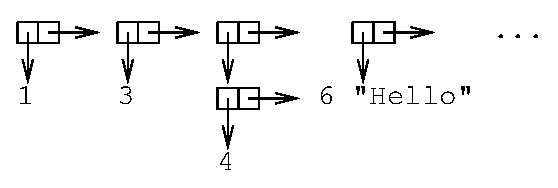
\includegraphics{inspect-as-cells}
\end{center}

\section{Extending Clouseau}

Sometimes Clouseau's built-in inspection abilities aren't enough, and
you want to be able to extend it to inspect one of your own classes in
a special way. Clouseau supports this, and it's fairly simple and
straightforward.

Suppose that you're writing a statistics program and you want to
specialize the inspector for your application. When you're looking at
a sample of some characteristic of a population, you want to be able
to inspect it and see some statistics about it, like the average. This
is easy to do.

We define a class for a statistical sample. We're keeping this very
basic, so it'll just contain a list of numbers:

\begin{alltt}
(in-package :clim-user)
(use-package :clouseau)

(defclass sample ()
  ((data :initarg :data
         :accessor data
         :type list :initform '()))
  (:documentation "A statistical sample"))

(defgeneric sample-size (sample)
  (:documentation "Return the size of a statistical sample"))

(defmethod sample-size ((sample sample))
  (length (data sample)))
\end{alltt}

The \genfun{print-object} function we define will print samples
unreadably, just showing their sample size. For example, a sample with
nine numbers will print as \texttt{\#<SAMPLE n=9>} We create such a
sample and call it \cl{*my-sample*}.

\begin{alltt}
(defmethod print-object ((object sample) stream)
  (print-unreadable-object (object stream :type t)
    (format stream "n=~D" (sample-size object))))

(defparameter *my-sample*
  (make-instance 'sample
                 :data '(12.8 3.7 14.9 15.2 13.66
                         8.97 9.81 7.0 23.092)))
\end{alltt}

We need some basic statistics functions. First, we'll do sum:

\begin{alltt}
(defgeneric sum (sample)
  (:documentation "The sum of all numbers in a statistical
sample"))

(defmethod sum ((sample sample))
  (reduce #'+ (data sample)))
\end{alltt}

Next, we want to be able to compute the mean. This is just the
standard average that everyone learns: add up all the numbers and
divide by how many of them there are. It's written $\overline{x}$.

\begin{alltt}
(defgeneric mean (sample) 
  (:documentation "The mean of the numbers in a statistical
sample"))

(defmethod mean ((sample sample))
  (/ (sum sample)
     (sample-size sample)))
\end{alltt}

Finally, to be really fancy, we'll throw in a function to compute the
standard deviation. You don't need to understand this, but the
standard deviation is a measurement of how spread out or bunched
together the numbers in the sample are. It's called $s$, and
it's computed like this:

$$ s = \sqrt{\frac{1}{N-1} \sum_{i=1}^N (x_i - \overline{x})^2} $$

\begin{alltt}
(defgeneric standard-deviation (sample)
  (:documentation "Find the standard deviation of the numbers
in a sample. This measures how spread out they are."))

(defmethod standard-deviation ((sample sample))
  (let ((mean (mean sample)))
    (sqrt (/ (loop for x in (data sample)
                   sum (expt (- x mean) 2))
             (1- (sample-size sample))))))
\end{alltt}

This is all very nice, but when we inspect \cl{*my-sample*} all we see
is a distinctly inconvenient display of the class, its superclass, and
its single slot, which we actually need to \emph{click on} to see. In
other words, there's a lot of potential being missed here. How do we
take advantage of it?

We can define our own inspection functions. To do this, we have two
methods that we can define. To change how sample objects are inspected
compactly, before they are clicked on, we can define an
\genfun{inspect-object-briefly} method for our \cl{sample} class. To
change the full, detailed inspection of samples, we define
\genfun{inspect-object} for the class. Both of these methods take two
arguments: the object to inspect and a CLIM output stream. They are
expected to print a representation of the object to the stream.

Because we defined \genfun{print-object} for the \cl{sample} class to
be as informative as we want the simple representation to be, we don't
need to define a special \genfun{inspect-object-briefly} method. We
should, however, define \genfun{inspect-object}.

\begin{alltt}
(defmethod inspect-object ((object sample) pane)
  (inspector-table (object pane)
      ;; This is the header
      (format pane "SAMPLE n=~D" (sample-size object))
    ;; Now the body
    (inspector-table-row (pane)
      (princ "mean" pane)
      (princ (mean object) pane))
    (inspector-table-row (pane)
      (princ "std. dev." pane)
      (princ (standard-deviation object) pane))))
\end{alltt}

Here, we introduce two new macros. \macro{inspector-table} sets up a
box in which we can display our representation of the sample. It
handles quite a bit of CLIM work for us. When possible, you should use
it instead of making your own, since using the standard facilities
helps ensure consistency.

The second macro, \macro{inspector-table-row}, creates a row with the
output of one form bolded on the left and the output of the other on
the right. This gives us some reasonably nice-looking output:

\begin{center}

\includegraphics{inspect-object-1}
\end{center}

But what we really want is something more closely adapted to our
needs. It would be nice if we could just have a table of things like
$ \overline{x} = 12.125776 $ and have them come out formatted
nicely. Before we attempt mathematical symbols, let's focus on getting
the basic layout right. For this, we can use CLIM's table formatting.

\begin{alltt}
(defmethod inspect-object ((object sample) pane)
  (flet ((x=y (x y)
           (formatting-row (pane)
             (formatting-cell (pane :align-x :right)
               (princ x pane))
             (formatting-cell (pane) (princ "=" pane))
             (formatting-cell (pane)
               (inspect-object y pane)))))
    (inspector-table (object pane)
        ;; This is the header
        (format pane "SAMPLE n=~D" (sample-size object))
      ;; Now the body
      (x=y "mean" (mean object))
      (x=y "std. dev." (standard-deviation object)))))
\end{alltt}

In this version, we define a local function \cl{x=y} which outputs a
row showing something in the form ``label = value''. If you look
closely, you'll notice that we print the label with \cl{princ} but we
print the value with \genfun{inspect-object}. This makes the value
inspectable, as it should be.

Then, in the \macro{inspector-table} body, we insert a couple of calls
to \cl{x=y} and we're done. It looks like this:

\begin{center}

\includegraphics{inspect-object-2}
\end{center}

Finally, for our amusement and further practice, we'll try to get some
mathematical symbols---in this case we'll just need $\overline{x}$. We
can get this by printing an italic $x$ and drawing a line over it:

\begin{alltt}
(defun xbar (stream)
  "Draw an x with a bar over it"
  (with-room-for-graphics (stream)
    (with-text-face (stream :italic)
      (princ \#\textbackslash{}x stream)
      (draw-line* stream 0 0
                  (text-style-width *default-text-style*
                                    stream) 0))))

(defmethod inspect-object ((object sample) pane)
  (flet ((x=y (x y)
           (formatting-row (pane)
             (formatting-cell (pane :align-x :right)
               ;; Call functions, print everything else in italic
               (if (functionp x)
                   (funcall x pane)
                   (with-text-face (pane :italic)
                     (princ x pane))))
             (formatting-cell (pane) (princ "=" pane))
             (formatting-cell (pane)
               (inspect-object y pane)))))
    (inspector-table (object pane)
        ;; This is the header
        (format pane "SAMPLE n=~D" (sample-size object))
      ;; Now the body
      (x=y \#'xbar (mean object))
      (x=y \#\textbackslash{}S (standard-deviation object)))))
\end{alltt}

Finally, to illustrate the proper use of
\genfun{inspect-object-briefly}, suppose that we want the ``n=9'' (or
whatever the sample size $n$ equals) part to have an itlicised $n$. We
can fix this easily:

\begin{alltt}
(defmethod inspect-object-briefly ((object sample) pane)
  (with-output-as-presentation (pane object 'sample)
    (with-text-family (pane :fix)
      (print-unreadable-object (object pane :type t)
        (with-text-family (pane :serif)
          (with-text-face (pane :italic)
            (princ "n" pane)))
        (format pane "=~D" (sample-size object))))))
\end{alltt}

Notice that the body of \genfun{inspect-object-briefly} just prints a
representation to a stream, like \genfun{inspect-object} but shorter.
It should wrap its output in \macro{with-output-as-presentation}.
\genfun{inspect-object} does this too, but it's hidden in the
\macro{inspector-table} macro.

Our final version looks like this:

\begin{center}

\includegraphics{inspect-object-3}
\end{center}

For more examples of how to extend the inspector, you can look at
\texttt{inspector.lisp}.

\section{API}

The following symbols are exported from the \cl{clouseau} package:

\defun {inspector} {object \key new-process}

Inspect \cl{object}. If \cl{new-process} is \cl{t}, Clouseau will be
run in a new process.

\defgeneric {inspect-object} {object pane}

Display inspected representation of \cl{object} to the extended output
stream \cl{pane}. This requires that \cl{*application-frame*} be bound
to an inspector application frame, so it isn't safe to use in other
applications.

\defgeneric {inspect-object-briefly} {object pane}

A brief version of \genfun{inspect-object}. The output should be
short, and should try to fit on one line.

\defgeneric {define-inspector-command} {name args \rest body}

This is just an inspector-specific version of
\genfun{define-command}. If you want to define an inspector command
for some reason, use this.

\defmacro {inspector-table} {(object pane) header \body body}

Present \cl{object} in tabular form on \cl{pane}, with \cl{header}
evaluated to print a label in a box at the top. \cl{body} should
output the rows of the table, possibly using \cl{inspector-table-row}.

\defmacro {inspector-table-row} {(pane) left right}

Output a table row with two items, produced by evaluating \cl{left}
and \cl{right}, on \cl{pane}. This should be used only within
\cl{inspector-table}.

When possible, you should try to use this and \cl{inspector-table} for
consistency, and because they handle quite a bit of effort for you.

\part{Auxiliary Material}

\chapter{Glossary}

\glossentry{Direct mirror}

A \gloss{mirror} of a sheet which is not shared with any of the
ancestors of the sheet.  All grafted McCLIM sheets have mirrors, but
not all have direct mirrors.  A McCLIM sheet that does not have a
direct mirror uses the direct mirror of its first ancestor having a
direct mirror for graphics output.  Asking for the direct mirror of a
sheet that does not have a direct mirror returns nil.

Whether a McCLIM sheet has a direct mirror or not, is decided by the
frame manager.  Some frame managers may only allow for the graft to be
a mirrored sheet.  Even frame managers that \emph{allow} hierarchical
mirrors may decide not to allocate a direct mirror for a particular
sheet.  Although sheets with a direct mirror must be instances of the
class mirrored-sheet-mixin, whether a McCLIM sheet has a direct mirror
or not is not determined statically by the class of a sheet, but
dynamically by the frame manager. 

\glossentry{Mirror}

A device window such as an X11 window that parallels a \gloss{sheet}
in the CLIM \gloss{sheet hierarchy}.  A \gloss{sheet} having such a
\emph{direct} mirror is called a \gloss{mirrored sheet}.  When
\gloss{drawing functions} are called on a \gloss{mirrored sheet}, they
are forwarded to the host windowing system as drawing commands on the
\gloss{mirror}.

CLIM \gloss{sheet}s that are not mirrored must be \gloss{descendents}
(direct or indirect) of a \gloss{mirrored sheet}, which will then be
the \gloss{sheet} that receives the drawing commands. 

\glossentry{Mirrored sheet}

A \gloss{sheet} in the CLIM \gloss{sheet hiearchy} that has a direct
parallel (called the \gloss{direct mirror}) in the host windowing
system.  A mirrored sheet is always an instance of the class
\class{mirrored-sheet-mixin}, but instances of that class are not
necessarily mirrored sheets.  The sheet is called a mirrored sheet
only if it currently has a direct mirror.  There may be several
reasons for an instance of that class not to currently have a direct
mirror.  One is that the sheet is not \gloss{grafted}.  Only grafted
sheets can have mirrors.  Another one is that the \gloss{frame
manager} responsible for the look and feel of the sheet hierarchy may
decide that it is inappropriate for the sheet to have a direct mirror,
for instance if the underlying windowing system does not allow nested
windows inside an application, or that it would simply be a better use
of resources not to create a direct mirror for the sheet.  An example
of the last example would be a stream pane inside a the
\gloss{viewport} of a \gloss{scroller pane}.  The graphics objects
(usually text) that appear in a stream pane can have very large
coordinate values, simply because there are many lines of text.
Should the stream pane be mirrored, the coordinate values used on the
mirror may easily go beyond what the underlying windowing system
accepts.  X11, for instance, can not handle coordinates greater than
64k (16 bit unsigned integer).  By not having a direct mirror for the
stream pane, the coordinates will be translated to those of the (not
necessarily direct) mirror of the \gloss{viewport} before being
submitted to the windowing system, which gives more reasonable
coordinate values.

It is important to realize the implications of this terminology.  A
mirrored sheet is therefore not a sheet that has a mirror.  All
grafted sheets have mirrors.  For the sheet to be a mirrored sheet it
has to have a \emph{direct} mirror.  Also, a call to
\genfun{sheet-mirror} returns a mirror for all grafted sheets, whether
the sheet is a mirrored sheet or not.  A call to
\genfun{sheet-direct-mirror}, on the other hand, returns nil if the
sheet is not a mirrored sheet. 

\glossentry{Mirror transformation}

The transformation that transforms coordinates in the coordinate
system of a mirror (i.e. the native coordinates of the mirror) to
native coordinates of its parent in the underlying windowing system.
On most systems, including X, this transformation will be a simple
translation. 

\glossentry{Native coordinates}

Each mirror has a coordinate system called the native coordinate
system.  Usually, the native coordinate system of a mirror has its
origin in the upper-left corner of the mirror, the x-axis grows to the
right and the y-axis downwards.  The unit is usually pixels, but the
frame manager can impose a native coordinate system with other units,
such as millimeters. 

The native coordinate system of a sheet is the native coordinate
system of its mirror (direct or not).  Thus, a sheet without a direct
mirror has the same native coordinate system as its parent.  To obtain
native coordinates of the parent of a mirror, use the \gloss{mirror
transformation}.

\glossentry{Native region}

The native region of a sheet is the intersection of its region and the
sheet region of all of its parents, expressed in the \gloss{native
coordinates} of the sheet. 

\glossentry{Potentially visible area}

A bounded area of an otherwise infinte drawing plane that is visible
unless it is covered by other visible areas. 

\glossentry{Sheet coordinates}

The coordinate system of coordinates obtained by application of the
\gloss{user transformation}.  

\glossentry{Sheet region}

The \gloss{region} of a sheet determines the visible part of the
drawing plane.  The dimensions of the sheet region are given in
\gloss{sheet coordinates}.  The location of the visible part of a
sheet within its \gloss{parent sheet} is determined by a combination
of the \gloss{sheet transformation} and the position of the sheet
region.

For instance, assuming that the sheet region is a rectangle with its
upper-left corner at (2, 1) and that the sheet transformation is a
simple translation (3, 2).  Then the origin of the \gloss{sheet
coordinate system} is at the point (3, 2) within the \gloss{sheet
coordinate system} of its \gloss{parent sheet}.  The origin of its the
coordinate system is not visible, however, because the visible region
has its upper-left corner at (2, 1) in the \gloss{sheet coordinate
system}.  Thus, the visible part will be a rectangle whose upper-left
corner is at (5, 3) in the \gloss{sheet coordinate system} of the
\gloss{parent sheet}.

Panes and gadgets alter the region and \gloss{sheet transformation} of
the underlying sheets (panes and gadgets are special kinds of sheets)
to obtain effects such as scrolling, zooming, coordinate system
transformations, etc.

\glossentry{Sheet transformation}

The transformation used to transform \gloss{sheet coordinates} of a
sheet to \gloss{sheet coordinates} of its \gloss{parent sheet}.  The
sheet transformation determine the position, shape, etc. of a sheet
within the coordinate system of its parent.

Panes and gadgets alter the transformation and \gloss{sheet region} of
the underlying sheets (panes and gadgets are special kinds of sheets)
to obtain effects such as scrolling, zooming, coordinate system
transformations, etc.

\glossentry{User Clipping region }

A \gloss{clipping region} used to limit the effect of \gloss{drawing
functions}.  The user \gloss{clipping region} is stored in the
\gloss{medium}.  It can be altered either by updating the
\gloss{medium}, or by passing a value for the :clipping-region
\gloss{drawing option} to a \gloss{drawing function}.

\glossentry{User Coordinates}

The coordinate system of coordinates passed to the \gloss{drawing
functions}.

\glossentry{User Transformation}

A transformation used to transform \gloss{user coordinates} into
\gloss{sheet coordinates}.  The user transformation is stored in the
\gloss{medium}.  It can be altered either by updating the
\gloss{medium}, or by passing a value for the :transformation
\gloss{drawing option} to a \gloss{drawing function}.


\glossentry{Visible area}

\chapter{Development History}

Mike McDonald started developing McCLIM in 1998.  His initial
objective was to be able to run the famous ``address book'' demo, and
to distribute the first version when this demo ran.  With this in
mind, he worked ``horizontally'', i.e., writing enough of the code for
many of the chapters of the specification to be able to run the
address book example.  In particular, Mike wrote the code for chapters
15 (Extended Stream Output), 16 (Output Recording), and 28
(Application Frames), as well as the code for interactor panes.  At
the end of 1999, Mike got too busy with other projects, and nothing
really moved.

Also in 1998, Gilbert Baumann started working ``vertically'', writing
a mostly-complete implementation of the chapters 3 (Regions) and 5
(Affine Transformations).  At the end of 1999, he realized that he was
not going to be able to finish the project by himself.  He therfore
posted his code to the free-CLIM mailing list.  Gilbert's code was
distributed according to the GNU Lesser General Public Licence (LGPL).

Robert Strandh picked up the project in 2000, starting from Gilbert's
code and writing large parts of chapters 7 (Properties of Sheets) and
8 (Sheet Protocols) as well as parts of chapters 9 (Ports, Grafts, and
Mirrored Sheets), 10 (Drawing Options), 11 (Text Styles), 12
(Graphics), and 13 (Drawing in Color).

In early 2000, Robert got in touch with Mike and eventually convinced him
to distribute his code, also according to the LGPL.  This was a major
turning point for the project, as the code base was now sufficiently
large that a number of small demos were actually running.  Robert
then spent a few months merging his code into that produced by Mike.

Arthur Lemmens wrote the initial version of the code for the gadgets
in june of 2000.

Bordeaux students Iban Hatchondo and Julien Boninfante were hired by
Robert for a 3-month summer project during the summer of 2000.  Their
objective was to get most of the pane protocols written (in particular
space composition and space allocation) as well as some of the gadgets
not already written by Arthur, in particular push buttons.  The
calculator demo was written to show the capabilities of their code.

In July of 2000, Robert invited Gilbert to the LSM-2000 metting in
Bordeaux (libre software meeting).  This meeting is a gathering of
developers of free software with the purpose of discussing strategy,
planning future projects, starting new ones, and working on existing
ones.  The main result of this meeting was that Gilbert managed to
merge his code for regions and transformations into the main code base
written by Mike, Robert, Iban, and Julien.  This was also a major step
towards a final system.  We now had one common code base, with a
near-complete implementation of regions, transformations, sheet
protocols, ports, grafts, graphics, mediums, panes, and gadgets.

Meanwhile, Mike was again able to work on the project, and during 2000
added much of the missing code for handling text interaction and
scrolling.  In particular, output recording could now be used to
redisplay the contents of an interactor pane.  Mike and Robert also
worked together to make sure the manipulation of sheet transformations
and sheet regions as part of scrolling and space-allocation respected
the specification.

Robert had initially planned for Iban and Julien to work on McCLIM for
their fifth-year student project starting late 2000 and continuing
until end of march 2001.  For reasons beyond his control, however, he
was forced to suggest a different project.  Thus, Iban and Julien,
together with two other students, were assigned to work on Gsharp, an
interactive score editor.  Gsharp was the original reason for Robert
to start working on CLIM as he needed a toolkit for writing a
graphical user interface for Ghsarp.  The lack of a freely-available
version of a widely-accepted toolkit such as CLIM made him decide to
give it a shot.  Robert's idea was to define the student project so
that a maximum of code could be written as part of McCLIM.  The result
was a complete rewrite of the space-allocation and space-composition
protocols, and many minor code snippets.

As part of the Gsharp project, Robert wrote the code for menu bars and
for a large part of chapter 27 (Command Processing).

Julien was hired for six months (April to September of 2001) by Robert
to make major progress on McCLIM.  Julien's first task was to create a
large demo that showed many of the existing features of McCLIM (a
``killer app'').  It was decided to use Gsharp since Julien was already
familiar with the application and since it was a sufficiently
complicated application that most of the features would be tested.  An
additional advantage of a large application was to serve as a ``smoke
test'' to run whenever substantial modifications to the code base had
been made.  As part of the Gsharp project, Julien first worked on
adding the possibility of using images as button labels.  

Early 2001, Robert had already written the beginning of a library for
manipulating 2-dimensional images as part of McCLIM.  A group of four
fourth-year students (Gregory Bossard, Michel Cabot, Cyrille Dindart,
Lionel Verg�) at the university of Bordeaux was assigned the task of
writing efficient code for displaying such images subject to arbitrary
affine transformations.  This code would be the base for drawing all
kinds of images such as icons and button labels, but also for an
application for manipulating document images.  The project lasted from
January to May of 2001.

Another group of four fourth-year students (Lo�c Lacomme, Nicolas
Louis, Arnaud Rouanet, Lionel Salabartan) at the university of
Bordeaux was assigned the task of writing a file-selector gadget
presented as a tree of directories and files, and with the ability to
open and close directories, to select files, etc.  The project lasted
from January to May of 2001.

One student in particular, Arnaud Rouanet started becoming interested
in the rest of CLIM as well.  During early 2001, he fixed several bugs
and also added new code, in particular in the code for regions,
graphics, and clx-mediums.

Arnaud and Lionel were hired by Robert for the summer of 2001 to work
on several things.  In particular, they worked on getting output
recording to work and wrote CLIM-fig, a demo that shows how output
recording is used.  They also worked on various sheet protocols, and
wrote the first version of the PostScript backend.

Alexey Dejneka joined the project in the summer of 2001. He wrote the
code for table formatting, bordered output and continued to develop
the PostScript output facility.

In the fall of 2001 Tim Moore became interested in the presentation
type system.  He implemented presentation type definition and
presentation method dispatch.  Wanting to see that work do something
useful, he went on to implement present and accept methods, extended
input streams, encapsulating streams, and the beginnings of input
editing streams.  In the spring of 2002 he wrote the core of Goatee,
an Emacs-like editor.  This is used to implement CLIM input editing.

Brian Spilsbury became involved towards the beginning of 2001.  His
motivation for getting involved was in order to have
internationalization support.  He quickly realized that the first step
was to make SBCL and CMUCL support Unicode.  He therefore worked to
make that happen.  So far (summer 2001) he has contributed a number of
cosmetic fixes to McCLIM and olos worked on a GTK-like gadget set.  He
finally started work to get the OpenGL backend operational. 

\end{document}
% LocalWords:  viewport scroller mixin} PostScript
